\documentclass[12pt, twoside]{article}
\usepackage[letterpaper, margin=1in, headsep=0.5in]{geometry}
\usepackage[english]{babel}
\usepackage[utf8]{inputenc}
\usepackage{amsmath}
\usepackage{amsfonts}
\usepackage{amssymb}
\usepackage{tikz}
%\usetikzlibrary{quotes, angles}

\usepackage{graphicx}
\usepackage{enumitem}
\usepackage{multicol}

\usepackage{fancyhdr}
\pagestyle{fancy}
\fancyhf{}
\renewcommand{\headrulewidth}{0pt} % disable the underline of the header

\fancyhead[R]{\thepage}
\fancyhead[L]{BECA / Dr. Huson / 10th Grade Geometry\\* Learning trajectory: Area, perimeter, volume}

\begin{document}
\subsubsection*{Area, perimeter, volume}
  \begin{enumerate}
  \item Rectangle, square area and perimeter
  \item Circle area and circumference
  \item Sector areas, arc length
  \item Solve for parameter versus calculate result
  \item Compound shapes (including margins)
  \item Distance on the coordinate plane
  \begin{enumerate}
    \item Plotting, labeling points, etc.
    \item Horizontal \& vertical distances
    \item Pythagorean formula
    \item Applications: Rhombus, isosceles $\triangle$,
    \item Radicals, $\pi$ and rounding
    \end{enumerate}
  \item Triangle area, perimeter (formula sheet)
  \item Volume: prism, cylinder, cone
  \item Surface area
  \item Scaling shapes (eg. rectangle, triangles including midline)
  \end{enumerate}

  \begin{enumerate}
    \subsubsection*{Basic shapes}
    \item Regents problems, January 2017, \#26, 34, 29?

\subsubsection*{Distance on the coordinate plane, proofs}

\item Triangle $ABC$ has vertices with coordinates A(,), B(,), and C(,). Prove that $\triangle ABC$ is an isoscelese triangle but not an equilateral triangle. (The use of the set of axes below is optional.)\\
Note: state both conclusions for full credit.

  \item Triangle $\triangle DAN$ is graphed on the set of axes below. The vertices of $\triangle DAN$ have the coordinates $T(-1,-2)$, $E(8,1)$, and $N(3,6)$.
    \begin{center} %4 quadrant regents grid
    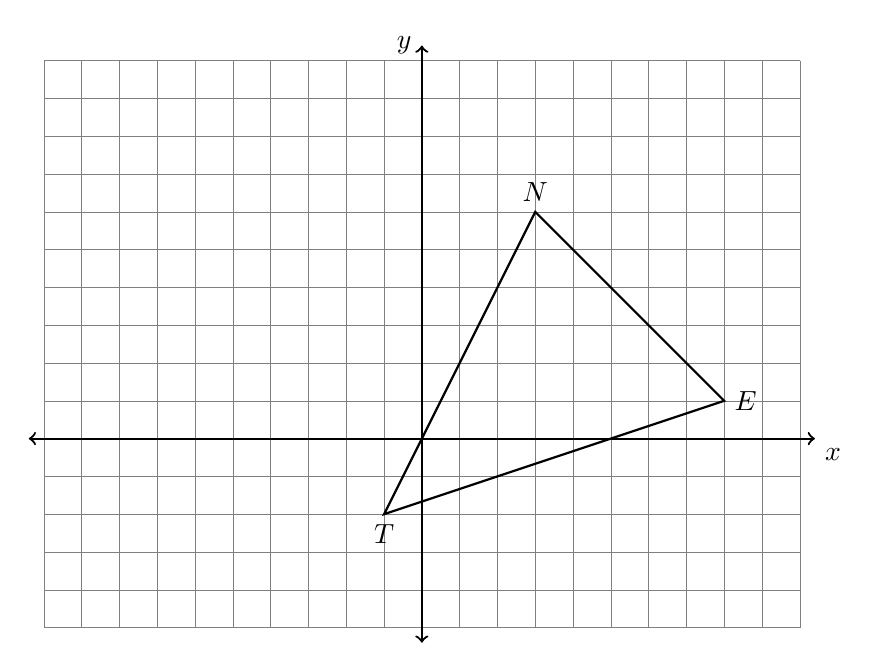
\begin{tikzpicture}[scale=.48]
      \draw [help lines] (-10,-5) grid (10,10);
      \draw [thick, <->] (-10.4,0) -- (10.4,0) node [below right] {$x$};
      \draw [thick, <->] (0,-5.4)--(0,10.4) node [left] {$y$};
      \draw [thick] (-1,-2) node[below] {$T$}--
      (8,1) node[right] {$E$}--
      (3,6) node[above] {$N$}--
      cycle;
      %\draw [fill] (5,0) circle [radius=0.1] node[above left] {$P$};
    \end{tikzpicture}
    \end{center}
    \begin{enumerate}
      \item Draw an altitude through point $N$ perpendicular to $\overline{TE}$.
      \item What is the length of the altitude drawn through $N$?
      \item What is the length of the base, $TE$?
      \item Find the area of  $\triangle DAN$.
    \end{enumerate}

  \item Given the quadrilateral $RSTU$ with $R(1,3)$, $S(4,7)$, $T(4,2)$, and $U(1,-2)$.
    \begin{enumerate}
      \item Plot and label $RSTU$ on the grid.
      \item Using the distance formula or otherwise, calculate $RS$, $ST$, $TU$, and $RU$.
      \item Definition: If a quadrilateral has four congruent sides, then it is a rhombus.\\[0.5cm]
      Prove that $RSTU$ is a rhombus.
    \end{enumerate}
    \begin{center} %4 quadrant regents grid
    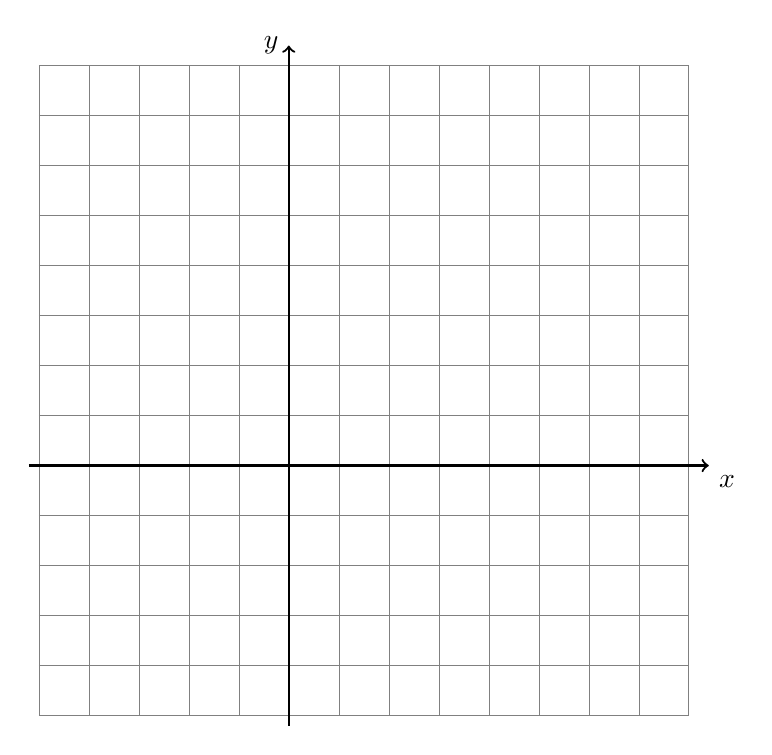
\begin{tikzpicture}[scale=.635]
      \draw [help lines] (-5,-5) grid (8,8);
      \draw [thick, ->] (-5.2,0) -- (8.4,0) node [below right] {$x$};
      \draw [thick, ->] (0,-5.2)--(0,8.4) node [left] {$y$};
    \end{tikzpicture}
    \end{center}

  \item Given the quadrilateral $RECT$ with $R(-4,1)$, $E(8,1)$, $C(8,6)$, and $T(-4,6)$.
    \begin{enumerate}
      \item Plot and label $RECT$ on the grid.
      \item Using the distance formula, calculate the length of the two diagonals $RC$ and $ET$.
      \item Theorem: If the diagonals of a quadrilateral are congruent, then it is a rectangle.\\[0.5cm]
      Prove that $RECT$ is a rectangle.
    \end{enumerate}
    \begin{center} %4 quadrant regents grid
    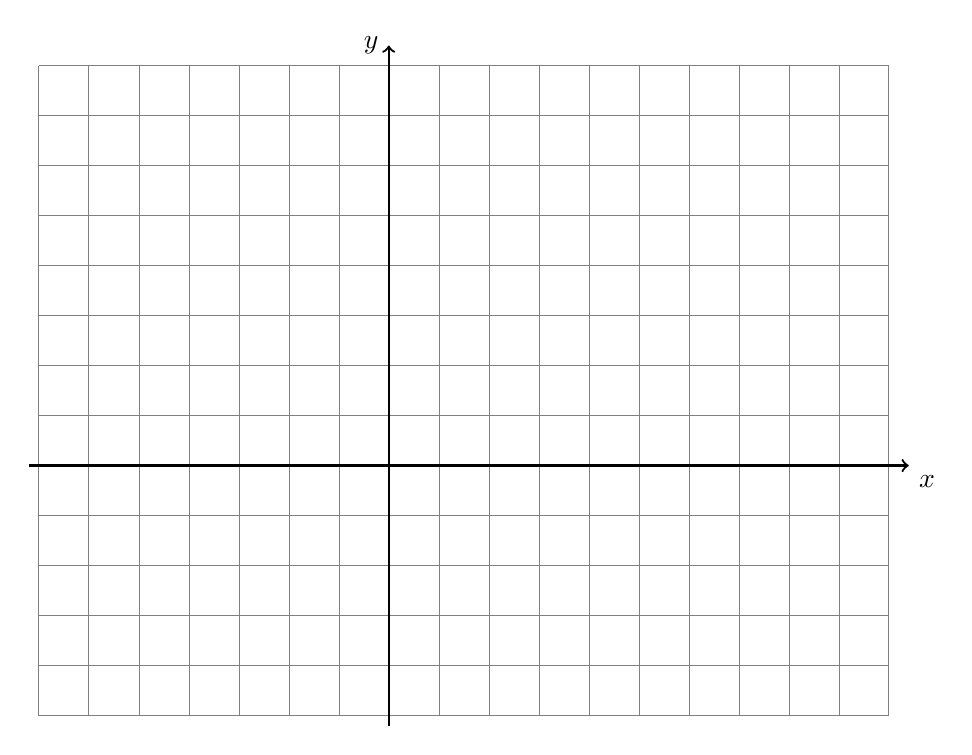
\begin{tikzpicture}[scale=.635]
      \draw [help lines] (-7,-5) grid (10,8);
      \draw [thick, ->] (-7.2,0) -- (10.4,0) node [below right] {$x$};
      \draw [thick, ->] (0,-5.2)--(0,8.4) node [left] {$y$};
    \end{tikzpicture}
    \end{center}

  \end{enumerate}

\end{document}
